% ============================================================================
\section{Introduction}
\label{sec:intro}
% ============================================================================

Multi-teacher on-policy distillation (MOPD) provides a practical way to
combine capabilities in one language model. The student generates responses,
and each response is scored by the teacher assigned to its task
\citep{ma2026mopdmultiteacheronpolicydistillation}. This allows specialist
teachers to be developed separately and their feedback to be combined during
student training. The same approach can add a new capability while using an
earlier model as a teacher to preserve existing ones
\citep{liu2026instella}. The intended outcome is a student that acquires
useful capabilities across tasks. A decrease in average teacher loss alone
does not establish that outcome.

Three questions must be distinguished. Can this student acquire each
capability through separate distillation? Can one shared model attain
those capability levels together? Can training reach them with the
available computation? Open-MOPD uses separately distilled students as
references and identifies capability imbalance in joint training
\citep{gao2026openmopddiagnosingfixingcapability}. These references establish
what the student learns separately; a gap in joint training can still
reflect task exposure, weak usable teacher signals, interacting updates,
or other optimization effects.

We study a local question about the training process:
\begin{quote}
Given capabilities that a student can acquire separately, when does a
shared MOPD update improve task objectives together, what limits its
rate, and when can more precise estimates help?
\end{quote}
Figure~\ref{fig:joint_progress_teaser} separates three cases. Exact,
nonconflicting updates can still make slow progress. A combined mean
gradient can oppose one task's loss gradient. Or a useful mean direction
can be estimated too imprecisely. Additional samples can improve precision;
under fixed task weights and optimizer scaling, they cannot change the
mean direction or its deterministic local rate.

\begin{figure}[t]
    \centering
    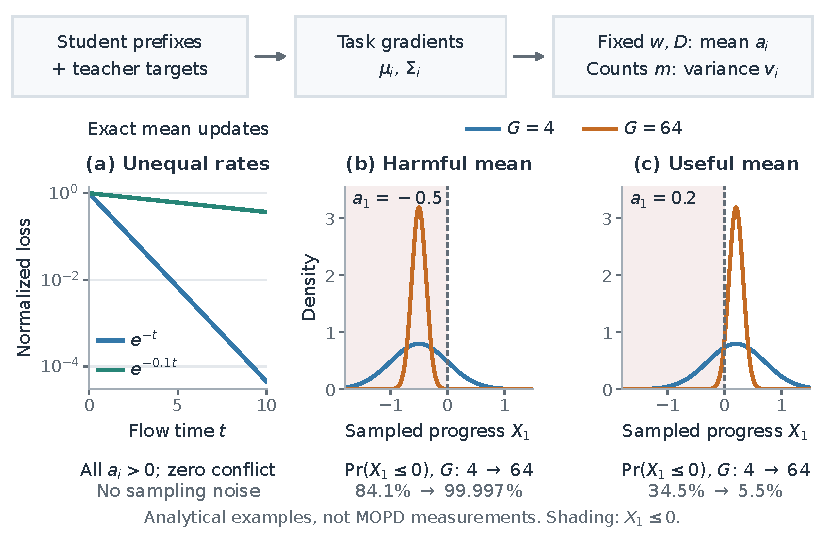
\includegraphics[width=\linewidth]{figures/joint_progress_teaser.pdf}
    \caption{Distinct limits on joint progress, illustrated analytically.
    (a) Orthogonal, noiseless task gradients yield unequal loss decay rates
    (Equation~\ref{eq:zero_conflict_rates}).
    (b,c) Sampling concentrates first-order progress $X_1$ around a harmful
    or useful mean. With $D=I$, $w_1=w_2=1/2$, independent Gaussian
    micro-batch gradients, $\Sigma_1=\Sigma_2=I$, and $m_1=m_2=G/2$,
    $X_1\sim\mathcal N(a_1,1/G)$. Set $\mu_1=(1,0)^\top$ and
    $\mu_2=(-2,1)^\top$ in (b), or $(-0.6,1)^\top$ in (c).
    Shading marks $X_1\leq0$. The sample-size comparison changes total
    budget $G$; GPAS instead reallocates a fixed budget and need not reduce
    every task's directional uncertainty. These are analytical examples,
    not measured MOPD results.}
    \label{fig:joint_progress_teaser}
\end{figure}

Existing work motivates testing these possible causes. CaMOPD studies counteracting
recovery and preservation gradients \citep{chen2026camopd}; D$^3$-MOPD
allocates samples using the remaining teacher gap and descent velocity
\citep{sun2026d3mopd}. Slow alignment has also been observed when the
training states are held fixed \citep{fu2026rethinkingopd2}. These findings
do not determine whether sampling uncertainty limits a particular MOPD
run. Dense top-$k$ supervision already computes multiple token
contributions at each prefix, while prompts and student trajectories
continue to produce variable gradients
\citep{ma2026mopdmultiteacheronpolicydistillation}.

We derive how teacher log-ratios on retained tokens produce task gradients,
then analyze the mean progress and directional uncertainty they imply.
A zero-conflict example separates common descent from fast learning;
a classical one-sided probability bound relates sampling to first-order
reliability. The analysis fixes the student-generated states and optimizer
scaling. We measure state-distribution changes and actual AdamW updates
separately. Local progress is a diagnostic; successful training can
temporarily increase a task loss.

Gradient-Preconditioned Adaptive Sampling (GPAS) provides an allocation
intervention for this analysis. It applies Neyman allocation to gradient
variance after optimizer scaling and preserves the specified task mean
weights. Its per-step rule minimizes an estimate of total update variance,
a conservative measure of uncertainty in task progress. We give an
analytical example in which the
variance-minimizing allocation has greater directional uncertainty than
another allocation. A four-domain protocol tests the diagnostics against
controlled updates, separately acquired capabilities, and end-to-end
training efficiency.
\missing{Replace the protocol contribution with measured findings after
the diagnostic and training comparisons are complete.}
